\chapter{Petri-hálók és alkalmazásaik}

\section{A Petri-hálók matematikai modellje}

A Petri-háló egy matematikai leírómodell elosztott rendszerek bemutatására.
A modellt Carl Adam Petri készítette.
A modell nagyon hasonlít a programozók körében elterjedt folyamat ábrára.
A háló irányított élekből, helyekből és átmenetekből (\textsl{mint elemek}) áll.
Az élek csak két különböző típusú elem között állhatnak.
A helyeken jelölő objektumok, úgynevezett tokenek állhatnak.
A tokenek csak diszkrét számban fordulhatnak elő egy helyen, és a token átvitele atomi folyamat, azaz nem félbeszakítható.
A tokenek elláthatóak attribútummal is, ilyen esetben a tokeneket "kiszínezzük" és színezett petri hálóról beszélünk. %TODO (LINK!)

%TODO cite: https://www.abhishekhalder.org/PetriNetReport.pdf__vq9vUXcOjS%2BawepkKcMLeAA64c19da3fb4d67754c3fe7eba8ce1187
A Petri háló alapvető matematikai modellje egy páros, irányított és súlyozott multigráf $PN(P,T,A,W,S)$, ahol 
\begin{itemize}
\item $P=\{ p_1,p_2,\ldots ,p_N \}$: a helyek véges halmaza,
\item $T=\{ t_1,t_2,\ldots ,t_M\}$: egy véges tranzició halmaz,
\item $P\cap T = \emptyset$,
\item $A \subseteq P\times T \cup T\times P$: az élek halmaza,
\item $W: F\Rightarrow N^+$: az élsúlyok halmaza,
\item $S: P\Rightarrow N^+$: a kezdőállapot.
\end{itemize}

\section{Színezett Petri-hálók}

Az elemi színezett háló felírható, mint egy
\[
CPN(P, T, A, \Sigma, V, C, G, E, S)
\]
struktúra, ahol 
\begin{itemize}
\item $P=\{ p_1, p_2, \ldots, p_N \}$: a helyek véges halmaza,
\item $T=\{ t_1, t_2, \ldots, t_M\}$: egy véges tranzició halmaz,
\item $A \subseteq P\times T \cup T \times P$: az élek halmaza,
\item $\Sigma$: a színek halmazainak halmaza, 
\item $V$: a változók halmaza, ahol $\forall v\in V$: változóhoz egy $Type[v] \in \Sigma $ típus rendelhető,
\item $C: P\rightarrow \Sigma$: a helyekhez színeket rendelő függvény,
\item $G: T\rightarrow EXPR_V$: az egyes tranzíciókhoz kapcsolódó validációs, ellenőrzési kifejezés (logikai értékű),
\item $E: A\rightarrow EXPR_V$: az egyes élekhez kapcsolódó kifejezés, amely a kapcsolódó hely színhalmazához tartozó értéket vehet fel,
\item $S: P\Rightarrow N^+$: a kezdőállapot.
\end{itemize}

Adott $CPN(P, T, A, \Sigma, V, C, G, E, S)$ színezett hálóhoz az alábbi kezelő funkciók köthetőek: 
\begin{itemize}
\item $M(p)$: a jelölő (\textit{marker}) függvény, melynek értéke a $p$ helyhez kapcsolódó tokenek halmaza (színezett Petri háló esetén az $M(p)$ elemek színeinek illeszkedni kell a $C(p)$ színhalmazhoz),
\item $M_0(p)$: helyek induló tokenkészlete,
\item $Var(t)$: a tranzíciók viselkedését leíró változók halmaza,
\item $b(v)$: az adott $v$ változó értékét megadó kifejezés, ahol $b(v) \in Type[v]$.
\end{itemize}

Egy $t$ tranzíció esetén a $Var(t)$ kifejezés a tranzícióhoz rendelt változók együttese, ahol a változók a $G(t)$ vagy $E$(a: t-hez kötődő él) kifejezésekben szerepelnek.
Az egyes esetekhez tartozó halmazok tehát az alábbiak.
\begin{equation*}
Var(t)=\begin{cases}
\{n,d\}, &\text{ha } t=SendPacket, \\
\{n,d,success\}, &\text{ha } t= TransmitPacket, \\
\{n,d,k,data\}, &\text{ha } t=ReceivePacket, \\
\{n,success\}, &\text{ha } t=TrancmitAck, \\
\{n,k\}, &\text{ha }t=ReceiveAck.
\end{cases}
\end{equation*}

A hálóban egy tranzíció akkor engedélyezett (\textit{ready}), ha a bemenő helyeknél a kívánt tokenszám megtalálható.
Jelölt hálók esetében:
\[
M'(p)=M(p)-I(p,t)+O(p,t): \forall p\in P,
\]
ahol 
\begin{itemize}
\item $I:F\Rightarrow N^+:$  bejövő áram, intenzitás
\item $O:F\Rightarrow N^+:$ kimenő áram. intenzitás
\end{itemize}

A hierarchikus CPN rendszerben az átláthatóság növelése érdekében összefogó modulokat is lehet alkalmazni. Egy modul más elemi egységek együttese, tárolója (\ref{fig:schema}. ábra).

\begin{figure}[h!]
\centering
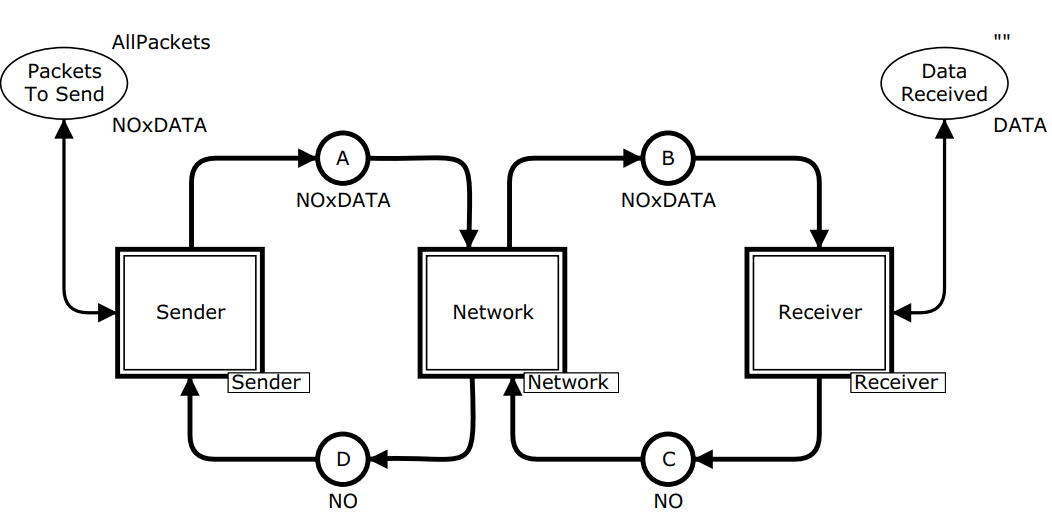
\includegraphics[scale=0.5]{images/rendszersema3modul.png}
\caption{Rendszerséma 3 modullal}
\label{fig:schema}
\end{figure}

A moduloknál fontos szerepet kapnak az átadó helyek, melyeken keresztül a tokenek bejöhetnek a modulba illetve kiléphetnek a modulból. Az ilyen port jellegű helyek lehetnek bemeneti portok (IN) illetve kimeneti portok (OUT).  

A CPN rendszerek egyik hasznos tulajdonsága, hogy lehetőséget adnak a felépített modell formális ellenőrzésére, validálására és értékelésére. A formális ellenőrzés egyik leggyakoribb eszköze az állapottér (\textit{state space})  modell, ahol az állapottér egy olyan irányított gráf, melyben a csomópontok a háló egy lehetséges  $M(CPN)$ jelölési állapota. Azaz a háló struktúrája rögzített, de az egyes elemeknél a tokenek és változók halmaza, azok állapota változhat. A véges állapottér modellt rendszerint szimulációkal állítják elő. 

Az állapottér modellből kiindulva további elemzésekre ad lehetőséget a komponens gráf modell (\textit{Strongly Connected Component Graph}, röviden SCC) formalizmus. Az SCC gráfból a rendszer általános viselkedési szabályaira lehet következtetni. Az SCC gráf olyan gráf, melynek csomópontjai az állapottér azon diszjunkt részhalmazai, ahol egy részhalmaz bármely két elemére igaz, hogy az egyik elem  elérhető a másikból. 

Az elemzések során az alábbi főbb tulajdonságok elemzésére szokás kitérni:
\begin{itemize}
\item Reachability Properties,
\item Boundedness Properties,
\item Home Properties,
\item Liveness Properties,
\item Fairness Properties.
\end{itemize}

